\section{Revisiting Galaktika after 16 years}

\margininbox{Galaktika}{
     \begin{citemize}
    \item Jack Hare
    \item Dave Wilson II
    \item Rhys Tyers
    \item Clare Tan
    \end{citemize}}{\explo}
    
\subsection{Getting to the Galaktika Shaft}

\passage[chamber]{Galaktika}! What a name, what a legend, what a place! The biggest chamber in the system by far, visited by only the oldest lags and featured at the beginning of the Hollow Mountain Vol. 1. Was it even real? Was it really as big? Having pondered these questions for years, we decided to find out.

A rare lack of keen freshers left Rhys, Clare and myself free to have a bimble by ourselves. Down, deep into \passage{M16} we went. The hangers are loose, the spits seized, and the rope thick and gritty.
The new bits (for me) in \passage{Ta Mokra} were impressive, with huge swings and lots of falling water. At the bottom, through a boulder choked rift, to a vast blackness, Rhys bolted down and announced this was not \passage[chamber]{Galaktika} – it was merely the prequel, the foreplay, the hint-of-what-was-to-come.

We climbed of house-sized stacked boulders, trying to find where to bolt down. Eventually we found the way, by hugging the left hand wall. Again Rhys bolted down, quickly fading from view and hearing. Clare and I settled in for a natter, until \bignote{Rhys' echoing voice informed us he was out of rope}.  It was either that, bolts, battery or courage, and rope was the most honourable way out. We left, taking photos, only 90 minutes to the surface.

\subsection{Onwards to Galaktika}

It took several days to organise a return to Galaktika. In that time, Davey Dubz and I returned to M16, rebolting much of the entrance series to replace some seriously scary spits. 

With that in place, Rhys, Davey and I made rapid progress down to \passage[chamber]{Galaktika} proper. Davey and I huddled in the shelter as Rhys bolted the final 5\,m down. Descending, I contemplated the vast scale of the shaft. It is roughly circular, some 70\,m deep and around 20\,m in diameter. The walls are smooth, though with loose flakes of rock, and the floor is littered with massive boulders.

\begin{marginfigure}
\frame{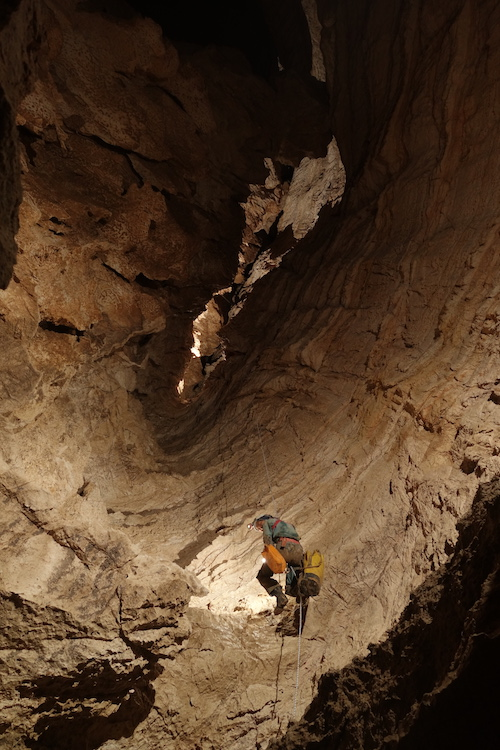
\includegraphics[width=\linewidth]{images/2017/jack-galaktika-2017/rhys_tamokra.jpg}}
\label{Ta Mokra}
\caption{Clare Tan on the impressive pitch on the way to the even more impressive \protect\passage[chamber]{Galaktika}\pic{Rhys Tyers}}
\end{marginfigure}



We regrouped, and looked for leads. At the lowest point of the chamber there was a promising crawl which went on for a while over soft mud, before choking with no way on. It lead towards the \passage[chamber]{Galaktika} Chamber. We returned to the shaft and found a potential lead --- crack in the wall by the water, blocked by a torso sized boulder.

We knew now that this was simply the shaft, and the chamber was next to it, separated by a large rock wall that extended half the depth of the shaft. We derigged the shaft as Rhys photographed us, and Davey kicked a huge flake of rock off which whistled silently past Rhys, only a few metres away. 

Rhys kindly let me rig down to the \passage[chamber]{Galaktika} chamber. However, dangling on the rope above the abyss, terrified for the obviously loose rock, I only placed one bolt before giving up, and let Rhys take over. Davey and I again sat in the humid, but warm shelter, listening to tunes as Rhys did all the hard work. Some exciting rigging later, involving sloping ledges and he was down to the dividing wall and out of rope.

I popped down with more rope and bolts. The swing across the to the top of the wall was immense, made more so by the further 30\,m or so of drop into the shaft below. I helpfully pointed out massive, unsupported boulders as Rhys rigged the final traverse and drop into the chamber.


\begin{figure}[t!]
\frame{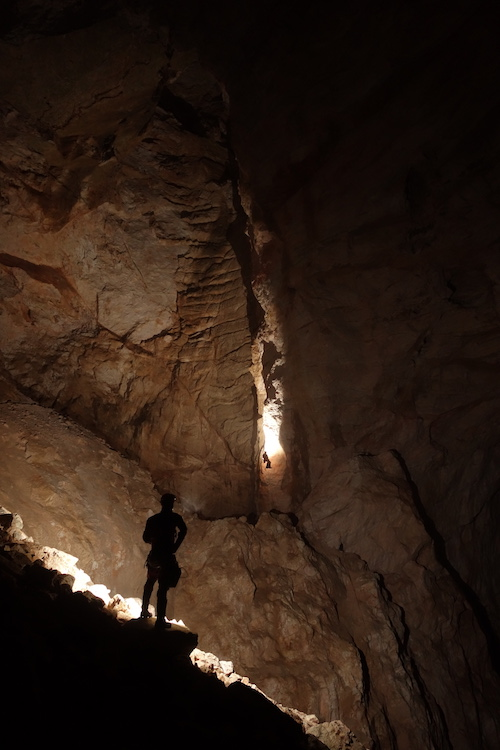
\includegraphics[width=\linewidth]{images/2017/jack-galaktika-2017/rhys-galaktika.jpg}}
\label{Ta Mokra}
\caption{   \protect\passage[chamber]{Galaktika} chamber is accessed by a large pendulum across the \protect\passage[shaft]{Galaktika} shaft \pic{Rhys Tyers}}
\end{figure}

\begin{marginsurvey}
\vspace{-400pt}
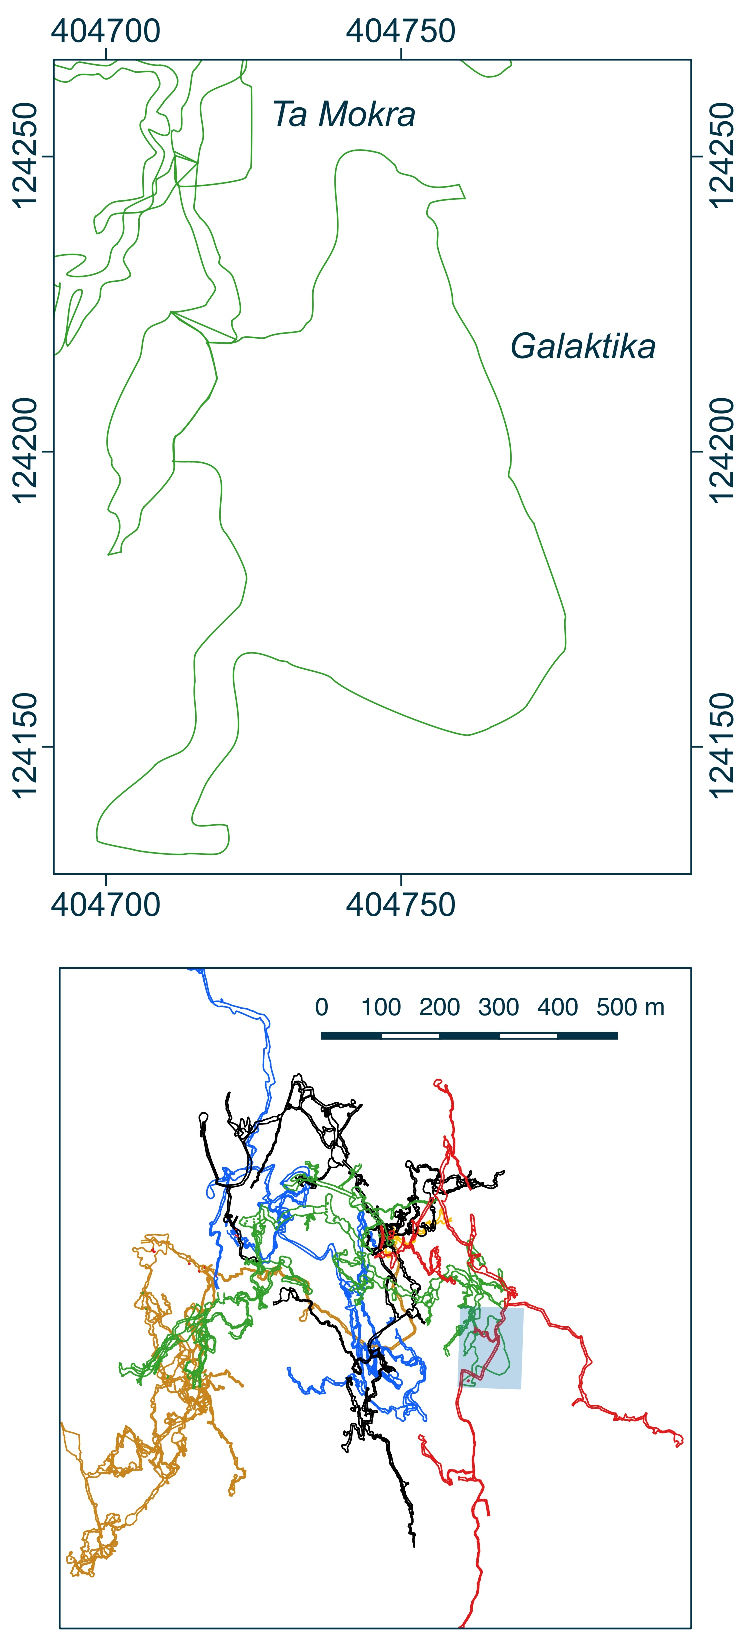
\includegraphics[width=\linewidth]{images/little_insets/galaktika_inset.pdf}
\label{Ta Mokra}
\caption[Galaktika chamber]{ Plan view of    \protect\passage[chamber]{Galaktika} chamber --- Slovenian National Grid EPSG 3794}
\end{marginsurvey}

The chamber is massive. I walked away from the others, and then sat in silence, watching them in the far distance, barely able to hear their voices. After circumnavigating the chamber (which takes 30 minutes or so) we met up, and Davey and I began to free climb down the boulder choke at the lowest point of the chamber. This is quite unpleasant, and at the bottom we found `ICCC 1994' spray painted on a wall, with no possible way on.

We found several fossilised turds, plum stones, grape stalks and all manner of archaeological evidence. Rhys took loads of great photos and we left in good time. The route is still rigged, and this is a superb cave for everyone to visit, from novices in training to old lags who want to revisit their glory days.

\name{Jack Hare}

\begin{pagefigure}
\frame{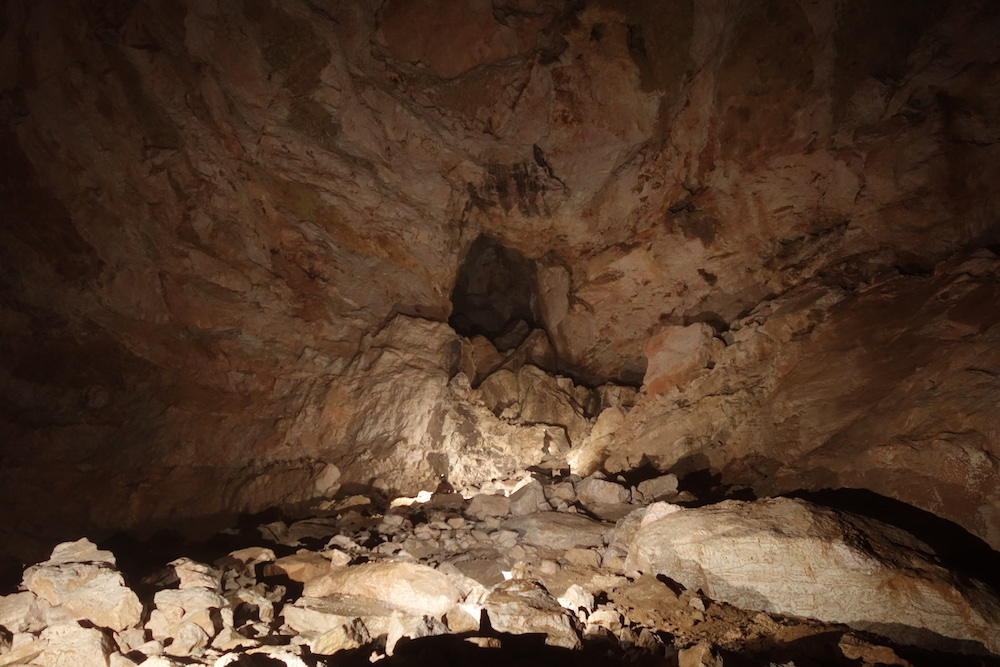
\includegraphics[width=\linewidth]{images/2017/jack-galaktika-2017/rhys-galaktika2.jpg}}
\label{Ta Mokra}
\caption{  Another view \protect\passage[chamber]{Galaktika} chamber showing a large, unclimbed aven on the southern side \pic{Rhys Tyers}}
\end{pagefigure}



